\documentclass{article} % For LaTeX2e
%\usepackage{nips14submit_e,times}
\usepackage{hyperref}
\usepackage{url}
\usepackage{amsmath,amsfonts,amsthm}

\usepackage{graphicx}
%\documentstyle[nips14submit_09,times,art10]{article} % For LaTeX 2.09

\usepackage{bm}
\def\B#1{\bm{#1}}
%\def\B#1{\mathbf{#1}}
\def\trans{\mathsf{T}}

%%%%%%%%%%%%%%%%%%%%%%%%%%%%%%%%%%%%%%%%%%%%%%%%%%%%%%%%%%%%%%%%%%%%%%%%%%%%%%%

\author{
DOHMATOB Elvis \inst[1]}
%% \institute{Parietal team, Inria Saclay Ile-de-France\\
%% Saclay, France\\

\title{A fast and simple primal-dual algorithm for computing Nash equilibria in two-person zero-sum games}


% The \author macro works with any number of authors. There are two commands
% used to separate the names and addresses of multiple authors: \And and \AND.
%
% Using \And between authors leaves it to \LaTeX{} to determine where to break
% the lines. Using \AND forces a linebreak at that point. So, if \LaTeX{}
% puts 3 of 4 authors names on the first line, and the last on the second
% line, try using \AND instead of \And before the third author name.

\newcommand{\fix}{\marginpar{FIX}}
\newcommand{\new}{\marginpar{NEW}}
\DeclareMathOperator{\prox}{prox}
\DeclareMathOperator{\im}{im}

\newtheorem{remark}{Remark}

\def \lb {{\langle}} \def \rb {{\rangle}}
\newcommand{\fro}[1]{\|#1\|_2}
\newcommand{\theHalgorithm}{\arabic{algorithm}}

\newcommand{\argmin}{\mathop{\mathrm{argmin}}}

\usepackage{hyperref}

\usepackage[ruled,vlined]{algorithm2e} \usepackage{framed}
\newtheorem{theorem}{Theorem} \newtheorem{lemma}[theorem]{Lemma}
\newtheorem{proposition}[theorem]{Proposition}
\newtheorem{corollary}[theorem]{Corollary}
\newtheorem{definition}[theorem]{Definition}

%\nipsfinalcopy % Uncomment for camera-ready version
%%%%%%%%%%%%%%%%%%%%%%%%%%%%%%%%%%%%%%%%%%%%%%%%%%%%%%%%%%%%%%%%%%%%%%%%%%%%%%%

\begin{document}


\maketitle

\begin{abstract}
We present a simple $\mathcal{O}(1/\epsilon)$ primal-dual algorithm with a low cost per iteration, for computing Nash equilibria in two-person zero-sum games. Our algorithm is applicable to a broad class of two-person zero-sum games including simultaneous games and sequential games with imcomplete information and perfect recall. The applicability to the latter kind of games is thanks to the sequence-form representation von Stengel's \cite{von1996efficient}. Our algorithm derives from the primal-dual algorithm developed by Chambolle and Pock in \cite{chambolle2010}, which has gained considerable success in the signal processing community, but is not directly applicable to the saddle-point problem corresponding to Nash equilibria, since the strategy profiles of players are sufficiently complex
% (for example, simplexes for simultaneous games, and intersections of hyperplanes and nonnegative orthants, for sequential games)
 to prevent easy computation 
% (i.e using non-iterative procedures, etc.)
of euclidean
% (metric)%
 projections thereupon (the proximal operators).
Our technique is to dualize the constraints in the Nash equilibrium problem, thus effectively unconstraining the problem. The resulting algorithm is simple, only involving matrix-vector multiplications
% (without any matrix inversions, etc.)
and nonnegative clipping.
% (taking point-wise max of a vector and 0)
The $\mathcal{O}(1/\epsilon)$ convergence rate of our algorithm derives explicitly from the general primal-dual algorithm in \cite{chambolle2010}. As proof of concept, we apply our algorithm to solve Kuhn Poker.
\end{abstract}

\section{Introduction}
\label{sec:intro}
Though \textit{Nash equilibrium} has become a novel way for solving two-person zero-sum games, the problem of computing Nash equilibria for large-scale two-person zero-sum games is still largely unsolved. Even though this problem is, in theory, amendable to classical tools like LCP (\textit{Linear Constraint Programming}), at least for sequential games with imcomplete information the game (e.g Texas Hold'em Poker) is exceedingly larger than what such programs can handle.
%% We will be needing the following notation: %%  The reader should lookup any standard textbook
%% %% (for example \cite{boyd2004}) on convex optimization for a tutorial introduction to these notions.
%% Viz,
%% \begin{itemize}
%% \item $\mathbb{R}^n$: $n$-dimensional real vector space;
%% \item $\mathbb{R}^{m \times n}$: \quad space of all $m$-by-$n$ real matrices;
%% \item $0_{m,n}$: $m$-by-$n$ matrix of zeros;
%% \item $(x)_+$: \quad component-wise maximum of a vector $x$ and 0;
%% \item $\mathbb{R}^n_+$: \quad $\{x \in \mathbb{R}^n|x = (x)_+\}$, the $n$-dimensional nonnegative orthant 
%% \item $i_C$: \quad indicator function of a convex set $C$;
%% % \item $\Pi_C$: \quad euclidean projection operator onto a convex set $C$;
%% \item $\|K\|_2$: \quad spectral norm of a matrix $K$
%% % \item $F^*$: the convex conjugate of a convex function $F$.
%% %% \item \textit{l.s.c.p.c}: \quad acronym for adjective \textit{lower semi-continuous proper convex};
%% %% \item $f^*$: \quad Fenchel transform (a.k.a convex conjugate) of a \textit{l.s.c.p.c} function $f$;
%% \end{itemize}

\section{Statement of the problem}
We are interested in computing Nash equilibria for \textit{two-person zero-sum} games. The problem takes the well-known \textit{minimax} form
\begin{equation}
  \underset{y \in Q_2}{minimize}\text{ }\underset{x \in Q_1}{maximize}\text{ }{x^TAy}
  \label{eq:opt_pb}
\end{equation}

where \textit{feasibility sets} $Q_j$ have the form
\begin{equation}
  Q_j := \{z \in C_j|E_jz = e_j\}
\end{equation}
for some convex subset $C_j$ of a euclidean space $\mathbb{R}^{n_j}$, and some vector $e_j \in \mathbb{R}^{p_j}$.
$Q_j$ is the \textit{strategy portfolio} for player $j$. $A$ is the \textit{payoff matrix} from player 1's perspective of the game: if player 1 players strategy
$x \in Q_1$ and player 2 plays strategy $y \in Q_2$ then player 1 gets $x^TAy$ units of money; that the game is ``zero-sum'' means that player 2 gets $-x^TAy$.
We will assume that the convex sets $C_j$ are simple enough so that the eucliean projection operators $\Pi_{C_j}$ can be cheaply computed.
Typically, $C_j = \mathbb{R}^{p_j}_+ := \{x \in \mathbb{R}^n|x_j \ge 0\}$, the \textit{the nonnegative orthant}, and encodes a nonnegativity constraint. %% in this case, $\Pi_{C_j}(z) \equiv (z)_+$ as seen in subsection \ref{sec:notation}.
As usual, the ``minimax'' notation in problem \eqref{eq:opt_pb} means that a pair $(x^*, y^*) \in Q_1 \times Q_2$ is a solution iff
\begin{equation}
  x^TAy^* \le x^TAy \le {x^*}^TAy, \forall (x, y) \in Q_1 \times Q_2
\end{equation}
Such pairs $(x^*, y^*)$ correspond to the Nash equilibria of the game, and ${x^*}^TAy^*$ is the \textit{value}
\footnote{This value is the same for every equilibrium pair $(x^*, y^*)$.} of the game.

We can distinguish two categories of such games, in terms of (non-)simultaneity of play.
\paragraph{Simultaneous two-person zero-sum games}
\label{subsec:example_games}
Here, the Nash equilibrium problem takes the form \eqref{eq:opt_pb} with $p_j = 1$, $C_j = \mathbb{R}^{p_j}_+$, $E_j = 1_{1, n_j}$,
  and $e_j = 1$, so that $Q_j$ is simply the probabability $n_j$-simplex $\Delta_{n_j}$. Each point in $\Delta_{n_j}$ corresponds to a \textit{mixed-strategy} for player $j$,
and represents a randomization on their \textit{pure-strategies} (corresponding to the vertices of their propability simplex $\Delta_{n_j}$).

\paragraph{Two-person zero-sum sequential games with imcomplete information and perfect recall}
It is now known, thanks to the \textit{sequence-form representaion}, that the Nash equilibrium problem for such games takes the form \eqref{eq:opt_pb}.

We recall that in the sequence-form representation of such games,  $E_j$ is a matrix whose
entries are $-1$, $0$, or $+1$, and $e_j := (1, 0, 0, ..., 0)$. We also recall that $E_1$ and $e_1$ (resp. $E_2$ and $e_2$)
encode linear constraints player 1's (resp. player 2's)  ``admissible'' \textit{realization plans} $x$ (resp. $y$).

\paragraph{Example of Nash equilibirum}
As an illustration, the pair $(x^*, y^*)$ given by
$x^* = (1, .478, .522, .174, .826)$ and
$y^* = (1, 1/2, 1/2)$ is a Nash equilibrium for the sequence-form game given by (not showing zero entries)\\
$A = \left(\begin{array}{ccc}
  &   &  \\
  &   &  \\
  & 1 & -1\\
  & -2 & 4\\
1 &   &  
\end{array}\right)$, $E_1 = \left(\begin{array}{ccccc}
  1 &   &   &   &  \\
  -1 & 1 & 1 &   &  \\
  -1 &   &   & 1 & 1
\end{array}\right)$,
$E_2 = \left(\begin{array}{ccc}
  1 &   &  \\
  -1 & 1 & 1
\end{array}\right)$, $e_1 = (1, 0, 0)$, and $e_2 = (1, 0)$.

\begin{remark}
  At least for sequential games, the matrices $A$, $E_1$, and $E_2$ are very large (can have upto billions of rows and columns) but very sparse too.
%% : $A$ will be sparse because a concrete sequential game will
%% typically have very few\footnote{Few, relative to the size of the game tree.} leafs, and only a few
%% combinations of sequences of moves of the players, will actually lead to a leaf (i.e. end the game);
%% $E$ and $F$ will be sparse because the kinks of possible sequences of moves of each player will
%% zig-zag between only a limited number of the player's information sets so that a move at an information set will
%% rarely\footnote{Relative to the number of information sets for the player.}  extend another information set.
This sparsity should be thoroughly exploited by a solver for problem \eqref{eq:opt_pb}.
\end{remark}

%% In section \ref{sec:related_work}, we give a brief overview of existing methods for solving \eqref{eq:opt_pb}.
%% We elaborate our proposed algorithm in section \ref{sec:algo}.

\section{Related work}
\label{sec:related_work}

Pending...

\section{Some prerequisite notions from convex analysis}
\label{sec:notation}
We will need the following notations and definitions in the sequel. Given positive integers $m$ and $n$, $\mathbb{R}^{m \times n}$ denotes
the space of all $m$-by-$n$ real matrices. $0_{m,n}$ denotes the $m$-by-$n$ matrix of zeros and $1_{m,n}$ denotes the $m$-by-$n$ matrix of ones.
%% $\mathbb{R}^n_+$ := $\{x \in \mathbb{R}^n|x_j \ge 0 \text{ }  \forall j\}$ is the $n$-dimensional \textit{nonnegative orthant}.

For a vector $x \in \mathbb{R}^n$, $\|x\|$ denotes the $2$-\textit{norm} of $x$ defined by $\|x\| := \sqrt{x^Tx}$.
$(x)_+$ denotes its point-wise maximum with 0. Note that $(x)_+ \in \mathbb{R}^n_+$.
For example, $((-2, \pi))_+ = (max(-2, 0), max(\pi, 0)) = (0, \pi)$. The \textit{spectral norm} of a matrix $K$,
denoted $\|K\|$, is defined to be the largest \textit{singular value} of $K$, i.e the largest \textit{eigen-value} of $K^TK$ (or equivalently, of $KK^T$).

Given a \textit{convex subset} $C$ of $\mathbb{R}^n$, $i_C$ denotes its \textit{indicator function} defined by
$i_C(x) = 0$ if $x \in C$ and $i_C(x) = +\infty$ otherwise. Note that $i_{C \cap D} = i_C + i_D$. The \textit{euclidean projection operator} onto $C$, denoted $\Pi_C$ is the function
$\Pi: \mathbb{R}^n \mapsto C$, which maps a point $x \in \mathbb{R}^n$ to the (necessarily unique) point $\Pi_C(x)$ of $C$ which is closed to $x$. Precisely,
\begin{equation}
  \Pi_C(x) := \underset{c \in C}{argimin}\text{ }\|c - x\|^2
\end{equation}
For example, $\Pi_{\mathbb{R}^n_+}(x) = (x)_+, \forall x \in \mathbb{R}^n$.

Let $f : \mathbb{R}^n \rightarrow [0, +\infty]$ be a \textit{proper convex lower semi-continous function} (\textit{p.c.l.s.c} for short), and $\tau$ a positive real number. The \textit{proximal operator} of $f$ of rank $\tau$,
denoted $\text{prox}_{\tau f}$ is the function which maps a point $x \in \mathbb{R}^n$ to the (necessarily unique) solution of the problem
\begin{equation}
  \underset{z \in \mathbb{R}^n}{argmin}\text{ }\frac{1}{2}\|z - x\|^2 + \tau f(z)
\end{equation}

It is easy to see that if $f$ is the indicator function of a convex set $C$, then $\text{prox}_{\tau f} = \Pi_C, \forall \tau > 0$. In this sense, proximal operators can be seen
as a generalization of euclidean projection operators.

\section{The algorithm}
We now derive our primal-dual algorithm for solving the Nash equilibrium problem \eqref{eq:opt_pb}. The algorithm can is an application of the general primal-dual algorithm proposed in \cite{chambolle2010}. Though this scheme has recently gained considerable popularity in the signal processing community \cite{gramfort-etal:2013a, dohmatob2014benchmarking}, to the best of our knowledge, this is the first time it is being applied to compute Nash equilibria.

\begin{theorem}
  The Nash equilibrium problem \eqref{eq:opt_pb} can be re-written in the equivalent unconstrained form
  
  \begin{equation}
    \underset{y \in \mathbb{R}^{n_2}, v\in \mathbb{R}^{p_1}}{minimize}\text{ }\underset{x \in \mathbb{R}^{n_1}, u \in \mathbb{R}^{p_2}}{maximize}
           {\begin{bmatrix}x\\u\end{bmatrix}^TK\begin{bmatrix}y\\v\end{bmatrix} + G(y, v) - H(x, u)}
           \label{eq:unconstrained_pb}
  \end{equation}

  where $v \in \mathbb{R}^{p_1}$ and $u \in \mathbb{R}^{p_2}$ are auxiliary variables and 
  \begin{equation}
    \left .
    \begin{split}
      K :=
      \left[
        \begin{array}{c|c}
          A & -E_1^T \\ \hline
          E_2 & 0_{p_2, p_1}
        \end{array}
        \right] \in \mathbb{R}^{(n_1 + p_2) \times (n_2 + p_1)} \\
      %%\begin{bmatrix}A \text{ } E_1^T\\ E_2 \text{ } 0\end{bmatrix} \in \mathbb{R}^{(n_2 + p_1) \times (n_1 + p_2)}\\
      G: \mathbb{R}^{n_2} \times \mathbb{R}^{p_1} \rightarrow [0, +\infty], (y, v) \mapsto i_{C_2}(y) + e_1^Tv\\
      H: \mathbb{R}^{n_1} \times \mathbb{R}^{p_2} \rightarrow [0, +\infty], (x, u) \mapsto i_{C_1}(x) + e_2^Tu
    \end{split}
    \right\}
    \label{eq:things}
  \end{equation}
  
  Moreover, $G$ and $H$ are \textit{p.c.l.s.c} and their proximal operators are given by
  \begin{equation}
    \left .
    \begin{split}
      \text{prox}_{\tau G} : \mathbb{R}^{n_2} \times \mathbb{R}^{p_1} &\rightarrow \mathbb{R}^{n_2} \times \mathbb{R}^{p_1}\\
      (y, v) &\mapsto (\Pi_{C_2}(y), v - \tau e_1)\\
    \end{split}
    \right\}
  \end{equation}

  and
  \begin{equation}
    \left .
    \begin{split}
      \text{prox}_{\sigma F}: \mathbb{R}^{n_1} \times \mathbb{R}^{p_2} &\rightarrow \mathbb{R}^{n_1} \times \mathbb{R}^{p_2}\\
      (x, u) &\mapsto (\Pi_{C_1}(x), u - \sigma e_2)
    \end{split}
    \right\}
  \end{equation}
  \label{thm:pd}
\end{theorem}

%% Theorem \ref{thm:pd}, can be interpreted as follows: 2 players $x$ (player 1)  and $y$ (player 2) go heads-on in a zero-sum game with payoff matrix $A$. Their strategy, profiles are $Q_1$ and $Q_2$ respectively, meaning that if player $j$ players a strategy which is outside $Q_j$ then they are panalized by inflicting an infinite loss yupon them. To remedy this, they recruit assistants $u$ and $v$, whose sole goal is to preven the ...
\begin{proof} First observe that $\forall (x, y) \in \mathbb{R}^{n_1} \times \mathbb{R}^{n_2}$, we have
  \begin{eqnarray*}
      -i_{Q_1}(x) = -i_{C_1}(x) + \underset{v \in \mathbb{R}^{p_1}}{min}\text{}{v^T(e_1 - E_1x)},
      \end{eqnarray*}
  and
\begin{eqnarray*}
  i_{Q_2}(y) = i_{C_2}(y) + \underset{u \in \mathbb{R}^{p_2}}{max}\text{}{u^T(E_2y - e_2)}
\end{eqnarray*}
  Thus,% problem \eqref{eq:opt_pb} is equivalent to
  \begin{eqnarray*}
    \begin{split}
      x^TAy - i_{Q_1}(x) + i_{Q_2}(y) &= x^TAy -i_{C_1}(x) + \underset{v \in \mathbb{R}^{p_1}}{min}\text{}{v^T(e_1 - E_1x)} + i_{C_2}(y) + \underset{u \in \mathbb{R}^{p_2}}{max}\text{}{u^T(E_2y - e_2)}\\
      &= \underset{v \in \mathbb{R}^{p_1}}{min}\text{ }\underset{u \in \mathbb{R}^{p_2}}{min}\text{ }x^TAy - x^TE_1^Tv + u^TE_2y + i_{C_2}(y) + e_1^Tv -(i_{C_1}(x) + e_2^Tu)\\
      &= \underset{v\in \mathbb{R}^{p_1}}{min}\text{ }\underset{u \in \mathbb{R}^{p_2}}{max}
      {\begin{bmatrix}x\\u\end{bmatrix}^TK\begin{bmatrix}y\\v\end{bmatrix} + G(y, v) - H(x, u)},
    \end{split}
  \end{eqnarray*}
where $K$, $G$, and $H$ are as given in \eqref{eq:things}.

Hence,
\begin{eqnarray*}
  \begin{split}
    \underset{y \in Q_2}{min}\text{ }\underset{x \in Q_1}{max}\text{ }x^TAy &=
    \underset{y \in \mathbb{R}^{n_2}}{min}\text{ }\underset{x \in \mathbb{R}^{n_1}}{max}\text{ }x^TAy - i_{Q_1}(x) + i_{Q_2}(y)\\
    &= \underset{y \in \mathbb{R}^{n_2}}{min}\text{ }\underset{x \in \mathbb{R}^{n_1}}{max}\text{ }
\underset{v\in \mathbb{R}^{p_1}}{min}\text{ }\underset{u \in \mathbb{R}^{p_2}}{max}
      {\begin{bmatrix}x\\u\end{bmatrix}^TK\begin{bmatrix}y\\v\end{bmatrix} + G(y, v) - H(x, u)}\\
    &= \underset{y \in \mathbb{R}^{n_2}}{min}\text{ }\underset{v\in \mathbb{R}^{p_1}}{min}\text{ }\underset{x \in \mathbb{R}^{n_1}}{max}\text{ }
\underset{u \in \mathbb{R}^{p_2}}{max}
      {\begin{bmatrix}x\\u\end{bmatrix}^TK\begin{bmatrix}y\\v\end{bmatrix} + G(y, v) - H(x, u)}\\
      &=     \underset{y \in \mathbb{R}^{n_2}, v\in \mathbb{R}^{p_1}}{min}\text{ }\underset{x \in \mathbb{R}^{n_1}, u \in \mathbb{R}^{p_2}}{max}
           {\begin{bmatrix}x\\u\end{bmatrix}^TK\begin{bmatrix}y\\v\end{bmatrix} + G(y, v) - H(x, u)}
  \end{split}
\end{eqnarray*}
Thus problem \eqref{eq:opt_pb} is equivalent to problem \eqref{eq:unconstrained_pb} as claimed.

About the proximal operators, indeed both $G$ and $F$ are separable sums of the indicator function of a convex set, whose prox is simply the euclidean projection operator onto the set,  and a linear transformation $z \mapsto a^Tz$ whose prox, at rank $\tau$, is simply $z \mapsto z - \tau a$.
\end{proof}
Now applying Algorithm 39 of \cite{chambolle2010} with $F := H^*$ (the \textit{convex conjugate} of $H$)
 to problem \eqref{eq:unconstrained_pb}, we Algorithm \ref{Tab:algo} for solving the original problem \eqref{eq:opt_pb}. The $\mathcal{O}(1/\epsilon)$ convergence rate of Algorothm \ref{Tab:algo} hails directly from Theorem 1 of \cite{chambolle2010}. Note that this convergence rate cannot be improved in the framework of \cite{chambolle2010}, since neither $G$ nor $H$ is \textit{uniformly convex}.


\begin{algorithm}[htb]
  \caption{$\mathcal{O}(1/\epsilon)$ Primal-dual algorithm for solving the Nash equilibrium problem \eqref{eq:opt_pb}}
  \textbf{require}
  \begin{itemize}
    \item the specification of a game $(A, E_1, E_2, e_1, e_2, C_1, C_2)$, where $A \in \mathbb{R}^{n_1 \times n_2}$,
  $E_1 \in \mathbb{R}^{p_1 \times n_1}$, $E_2 \in \mathbb{R}^{p_2 \times n_2}$, $e_1 \in \mathbb{R}^{p_1}$, $e_2 \in \mathbb{R}^{p_2}$, $C_j$ is a convex subset of $\mathbb{R}^{n_j}$;
      \item a tolerance level $\epsilon > 0$, on the duality gap
  \end{itemize}
  \textbf{precompute} $\|K\|^2$, where $K$ is constructed as in equations \eqref{eq:unconstrained_pb}. $\|K\|^2$ can be computed via a \textit{power iteration} on $K^TK$, for example.\\
  \textbf{initialize}
  $x^{(0)} \in \mathbb{R}^{n_1}$; $v \in \mathbb{R}^{p_1}$; $\tilde{y^{(0)}}, y^{(0)} \in \mathbb{R}^{n_2}$; $u^{(0)} \in \mathbb{R}^{p_2}$; 
  $\tau, \sigma > 0 \text{ s.t. }\tau\sigma \|K\|^2 < 1$ (for example take $\tau = \sigma = .99/\|K\|$); $k = 0$.\\
  \Repeat{$\dfrac{\| x^{(k+1)} - x^{(k)}\|^2 + \|v^{(k+1)}- v^{(k)}\|^2}{\sigma} + \dfrac{\|y^{(k+1)}- y^{(k)}\|^2 + \|u^{(k+1)}- u^{(k)}\|^2}{\tau} < \epsilon$}{
    \begin{eqnarray*}
      x^{(k+1)} &\leftarrow& \Pi_{C_1}\left(x^{(k)} + \tau \left(A\tilde{y}^{(k)} - E_1^T\tilde{v}^{(k)}\right)\right)\\
      u^{(k+1)} &\leftarrow& u^{(k)} + \tau \left(E_2\tilde{y}^{(k)} - e_2\right)\\
      y^{(k+1)} &\leftarrow& \Pi_{C_2}\left(y^{(k)} - \sigma \left(A^Tx^{(k + 1)} + E_2^Tu^{(k + 1)}\right)\right)\\
      v^{(k+1)} &\leftarrow& v^{(k)} - \sigma \left(e_1 - E_1x^{(k+1)}\right)\\
      \tilde{y}^{(k+1)} &\leftarrow& 2y^{(k+1)} - y^{(k)}\\
      \tilde{u}^{(k+1)} &\leftarrow& 2u^{(k+1)} - u^{(k)}\\
      k &\leftarrow& k + 1
    \end{eqnarray*}
  } \Return $x^{(k)}$, $y^{(k)}$
  \label{Tab:algo}
\end{algorithm}

\subsection{Special case: $C_j = \mathbb{R}^{n_j}_+$} As discussed in subsection \ref{subsec:example_games},
the Nash equilibrium problem for two-person zero-sum simultaneous games and two-person zero-sum sequential games with imcomplete
information and perfect recall admits the formulation \eqref{eq:opt_pb}, with $C_j = \mathbb{R}^{n_j}_+$ (coding for nonnegativity constraints).
In such situations, $\Pi_{C_j}(z) \equiv (z)_+$ as already mentioned in \ref{sec:notation}, and Algorithm \ref{Tab:algo} reduces to the simpler Algorithm \ref{Tab:algo_simplified}.

\begin{algorithm}[htb]
  \caption{$\mathcal{O}(1/\epsilon)$ Primal-dual algorithm for solving the Nash equilibrium problem \eqref{eq:opt_pb}, with nonnegativity constraints $C_j = \mathbb{R}^{n_j}_+$}
  \textbf{require}
  \begin{itemize}
    \item the specification of a game $(A, E_1, E_2, e_1, e_2)$, where $A \in \mathbb{R}^{n_1 \times n_2}$,
  $E_1 \in \mathbb{R}^{p_1 \times n_1}$, $E_2 \in \mathbb{R}^{p_2 \times n_2}$, $e_1 \in \mathbb{R}^{p_1}$, $e_2 \in \mathbb{R}^{p_2}$;
      \item a tolerance level $\epsilon > 0$
  \end{itemize}
  \textbf{precompute} $\|K\|^2$, where $K$ is constructed as in equations \eqref{eq:unconstrained_pb}. $\|K\|^2$ can be computed via a \textit{power iteration} on $K^TK$, for example.\\
  \textbf{initialize}
  $x^{(0)} \in \mathbb{R}^{n_1}$; $v \in \mathbb{R}^{p_1}$; $\tilde{y^{(0)}}, y^{(0)} \in \mathbb{R}^{n_2}$; $u^{(0)} \in \mathbb{R}^{p_2}$; 
  $\tau, \sigma > 0 \text{ s.t. }\tau\sigma \|K\|^2 < 1$ (for example take $\tau = \sigma = .99/\|K\|$); $k = 0$.\\
  \Repeat{$\dfrac{\| x^{(k+1)} - x^{(k)}\|^2 + \|v^{(k+1)}- v^{(k)}\|^2}{\sigma} + \dfrac{\|y^{(k+1)}- y^{(k)}\|^2 + \|u^{(k+1)}- u^{(k)}\|^2}{\tau} < \epsilon$}{
    \begin{eqnarray*}
      x^{(k+1)} &\leftarrow& \left(x^{(k)} + \tau \left(A\tilde{y}^{(k)} - E_1^T\tilde{v}^{(k)}\right)\right)_+\\
      u^{(k+1)} &\leftarrow& u^{(k)} + \tau \left(E_2\tilde{y}^{(k)} - e_2\right)\\
      y^{(k+1)} &\leftarrow& \left(y^{(k)} - \sigma \left(A^Tx^{(k + 1)} + E_2^Tu^{(k + 1)}\right)\right)_+\\
      v^{(k+1)} &\leftarrow& v^{(k)} - \sigma \left(e_1 - E_1x^{(k+1)}\right)\\
      \tilde{y}^{(k+1)} &\leftarrow& 2y^{(k+1)} - y^{(k)}\\
      \tilde{u}^{(k+1)} &\leftarrow& 2u^{(k+1)} - u^{(k)}\\
      k &\leftarrow& k + 1
    \end{eqnarray*}
  } \Return $x^{(k)}$, $y^{(k)}$
  \label{Tab:algo_simplified}
\end{algorithm}


\section{Application to Poker: Kuhn Poker}
The Kuhn 3-card Poker has sequence-form specification given by (not showing zero entries)\\
$A = \left(\begin{array}{ccccccccccccc}
  &   &   &   &   &   &   &   &   &   &   &   &  \\
  &   &   &   &   &   &   & -1 / 6 &   &   &   & -1 / 6 &  \\
  &   &   &   &   &   &   &   & -1 / 6 &   &   &   & -1 / 6\\
  &   &   &   &   &   &   &   & -1 / 3 &   &   &   & -1 / 3\\
  &   &   &   &   & 1 / 6 & -1 / 3 &   &   & 1 / 6 & -1 / 3 &   &  \\
  &   &   & 1 / 6 &   &   &   &   &   &   &   & -1 / 6 &  \\
  &   &   &   & -1 / 6 &   &   &   &   &   &   &   & -1 / 6\\
  &   &   &   & 1 / 3 &   &   &   &   &   &   &   & -1 / 3\\
  & 1 / 6 & 1 / 3 &   &   &   &   &   &   & 1 / 6 & -1 / 3 &   &  \\
  &   &   & 1 / 6 &   &   &   & 1 / 6 &   &   &   &   &  \\
  &   &   &   & -1 / 6 &   &   &   & -1 / 6 &   &   &   &  \\
  &   &   &   & 1 / 3 &   &   &   & 1 / 3 &   &   &   &  \\
  & 1 / 6 & 1 / 3 &   &   & 1 / 6 & 1 / 3 &   &   &   &   &   &  
\end{array}\right)$,\\
$E_1 = \left(\begin{array}{ccccccccccccc}
1 &   &   &   &   &   &   &   &   &   &   &   &  \\
-1 &   &   &   &   &   &   &   &   & 1 &   &   & 1\\
-1 & 1 &   &   & 1 &   &   &   &   &   &   &   &  \\
-1 &   &   &   &   & 1 &   &   & 1 &   &   &   &  \\
  & -1 & 1 & 1 &   &   &   &   &   &   &   &   &  \\
  &   &   &   &   & -1 & 1 & 1 &   &   &   &   &  \\
  &   &   &   &   &   &   &   &   & -1 & 1 & 1 &  
\end{array}\right)$, $e_1 = e_2 = (1, 0, 0, 0, 0, 0, 0)$,\\
and $E_2 = \left(\begin{array}{ccccccccccccc}
1 &   &   &   &   &   &   &   &   &   &   &   &  \\
-1 &   &   &   &   &   &   & 1 & 1 &   &   &   &  \\
-1 &   &   &   &   &   &   &   &   & 1 & 1 &   &  \\
-1 &   &   &   &   & 1 & 1 &   &   &   &   &   &  \\
-1 &   &   &   &   &   &   &   &   &   &   & 1 & 1\\
-1 & 1 & 1 &   &   &   &   &   &   &   &   &   &  \\
-1 &   &   & 1 & 1 &   &   &   &   &   &   &   &  
\end{array}\right)$.\\
The pair $(x^*, y^*)$ of realization plans given by\\
$x^* = (1, 0.759, 0.759, 0, 0.241, 1, 0.425, 0.575, 0, 0.275, 0, 0.275, 0.725)$ and
$y^* = (1, 1, 0, 0.667, 0.333, 0.667, 0.333, 1, 0, 0, 1, 0, 1)$ is a Nash equlibrium for the game, computed using Algorithm  \ref{Tab:algo_simplified}. The convergence curve is shown in Fig \ref{Tab:conv_curves}. One easy checks that this equilibrium is feasible. Indeed,  $E_1x^* - e_1 = (4.76 \times 10^{-5}, -1.91 \times 10^{-5}, 5.67 \times 10^{-5}, 8.23 \times 10^{-6}, 2.90 \times 10^{-5}, -8.62 \times 10^{-7}, -1.96 \times 10^{-5})$ and $E_2y^* - e_2 = (-7.04 \times 10^{-7}, 2.27 \times 10^{-6}, -3.29 \times 10^{-6}, -1.50 \times 10^{-6}, 2.92 \times 10^{-6}, -4.97 \times 10^{-7}, -5.85 \times 10^{-7})$. Finally, $x^*TAy^* = -0.055593685705289997$, which agrees to 4 d.p with the value of $-1 / 18$ computed analytically by Kuhn in his 1954 paper.

\begin{figure}
  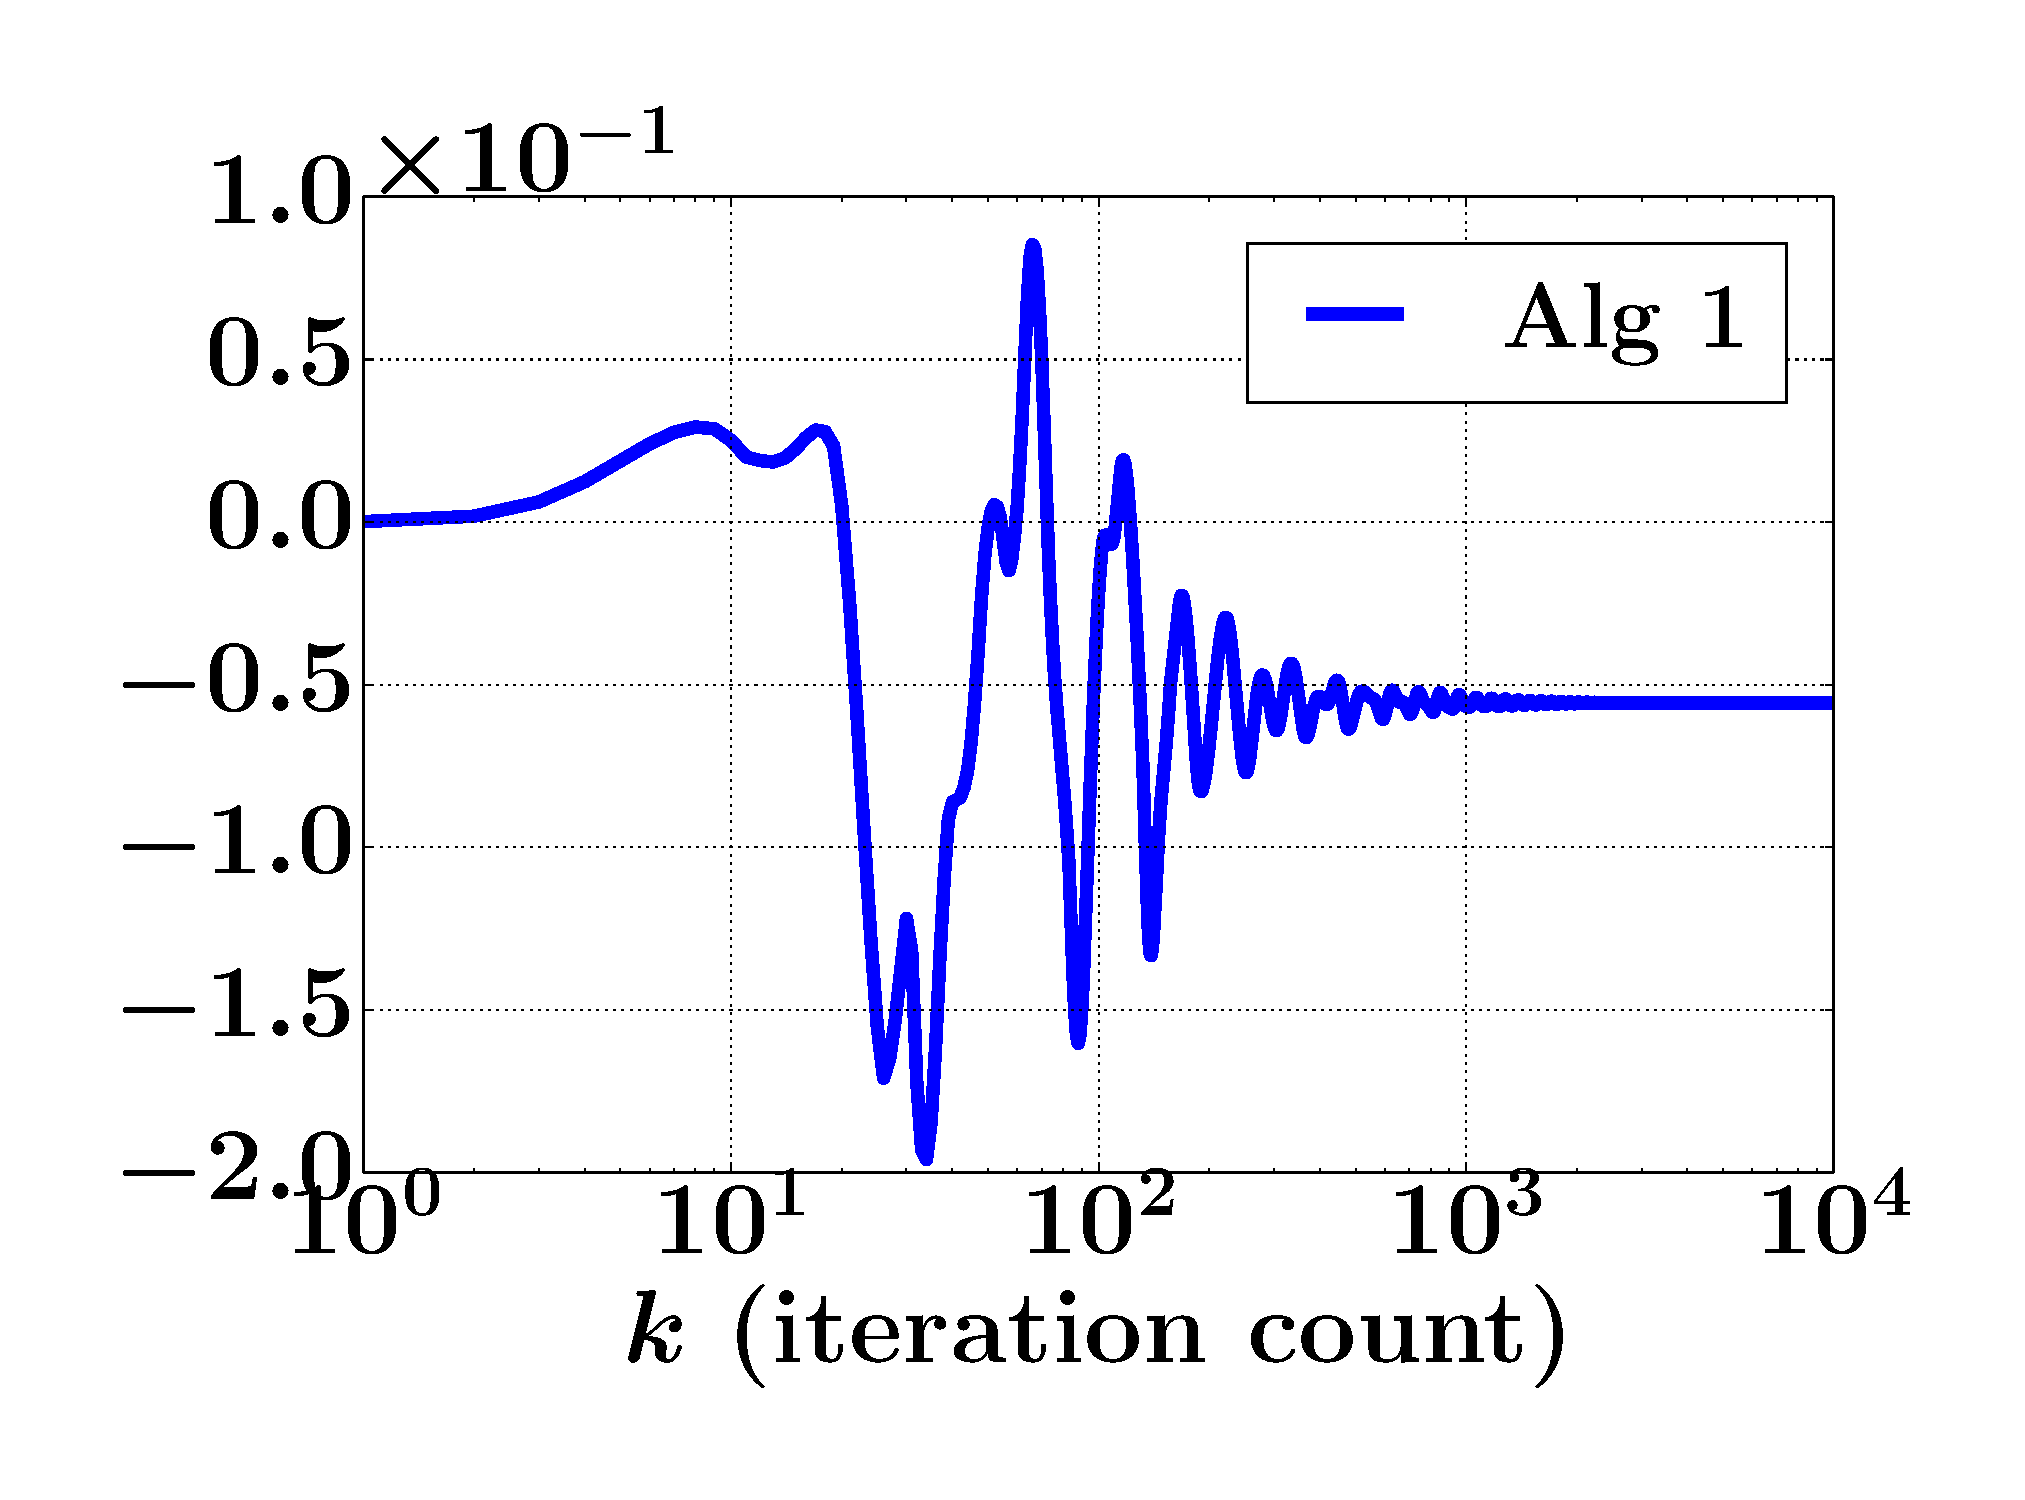
\includegraphics[width=.5\linewidth]{Kuhn3112_NE.pdf}
  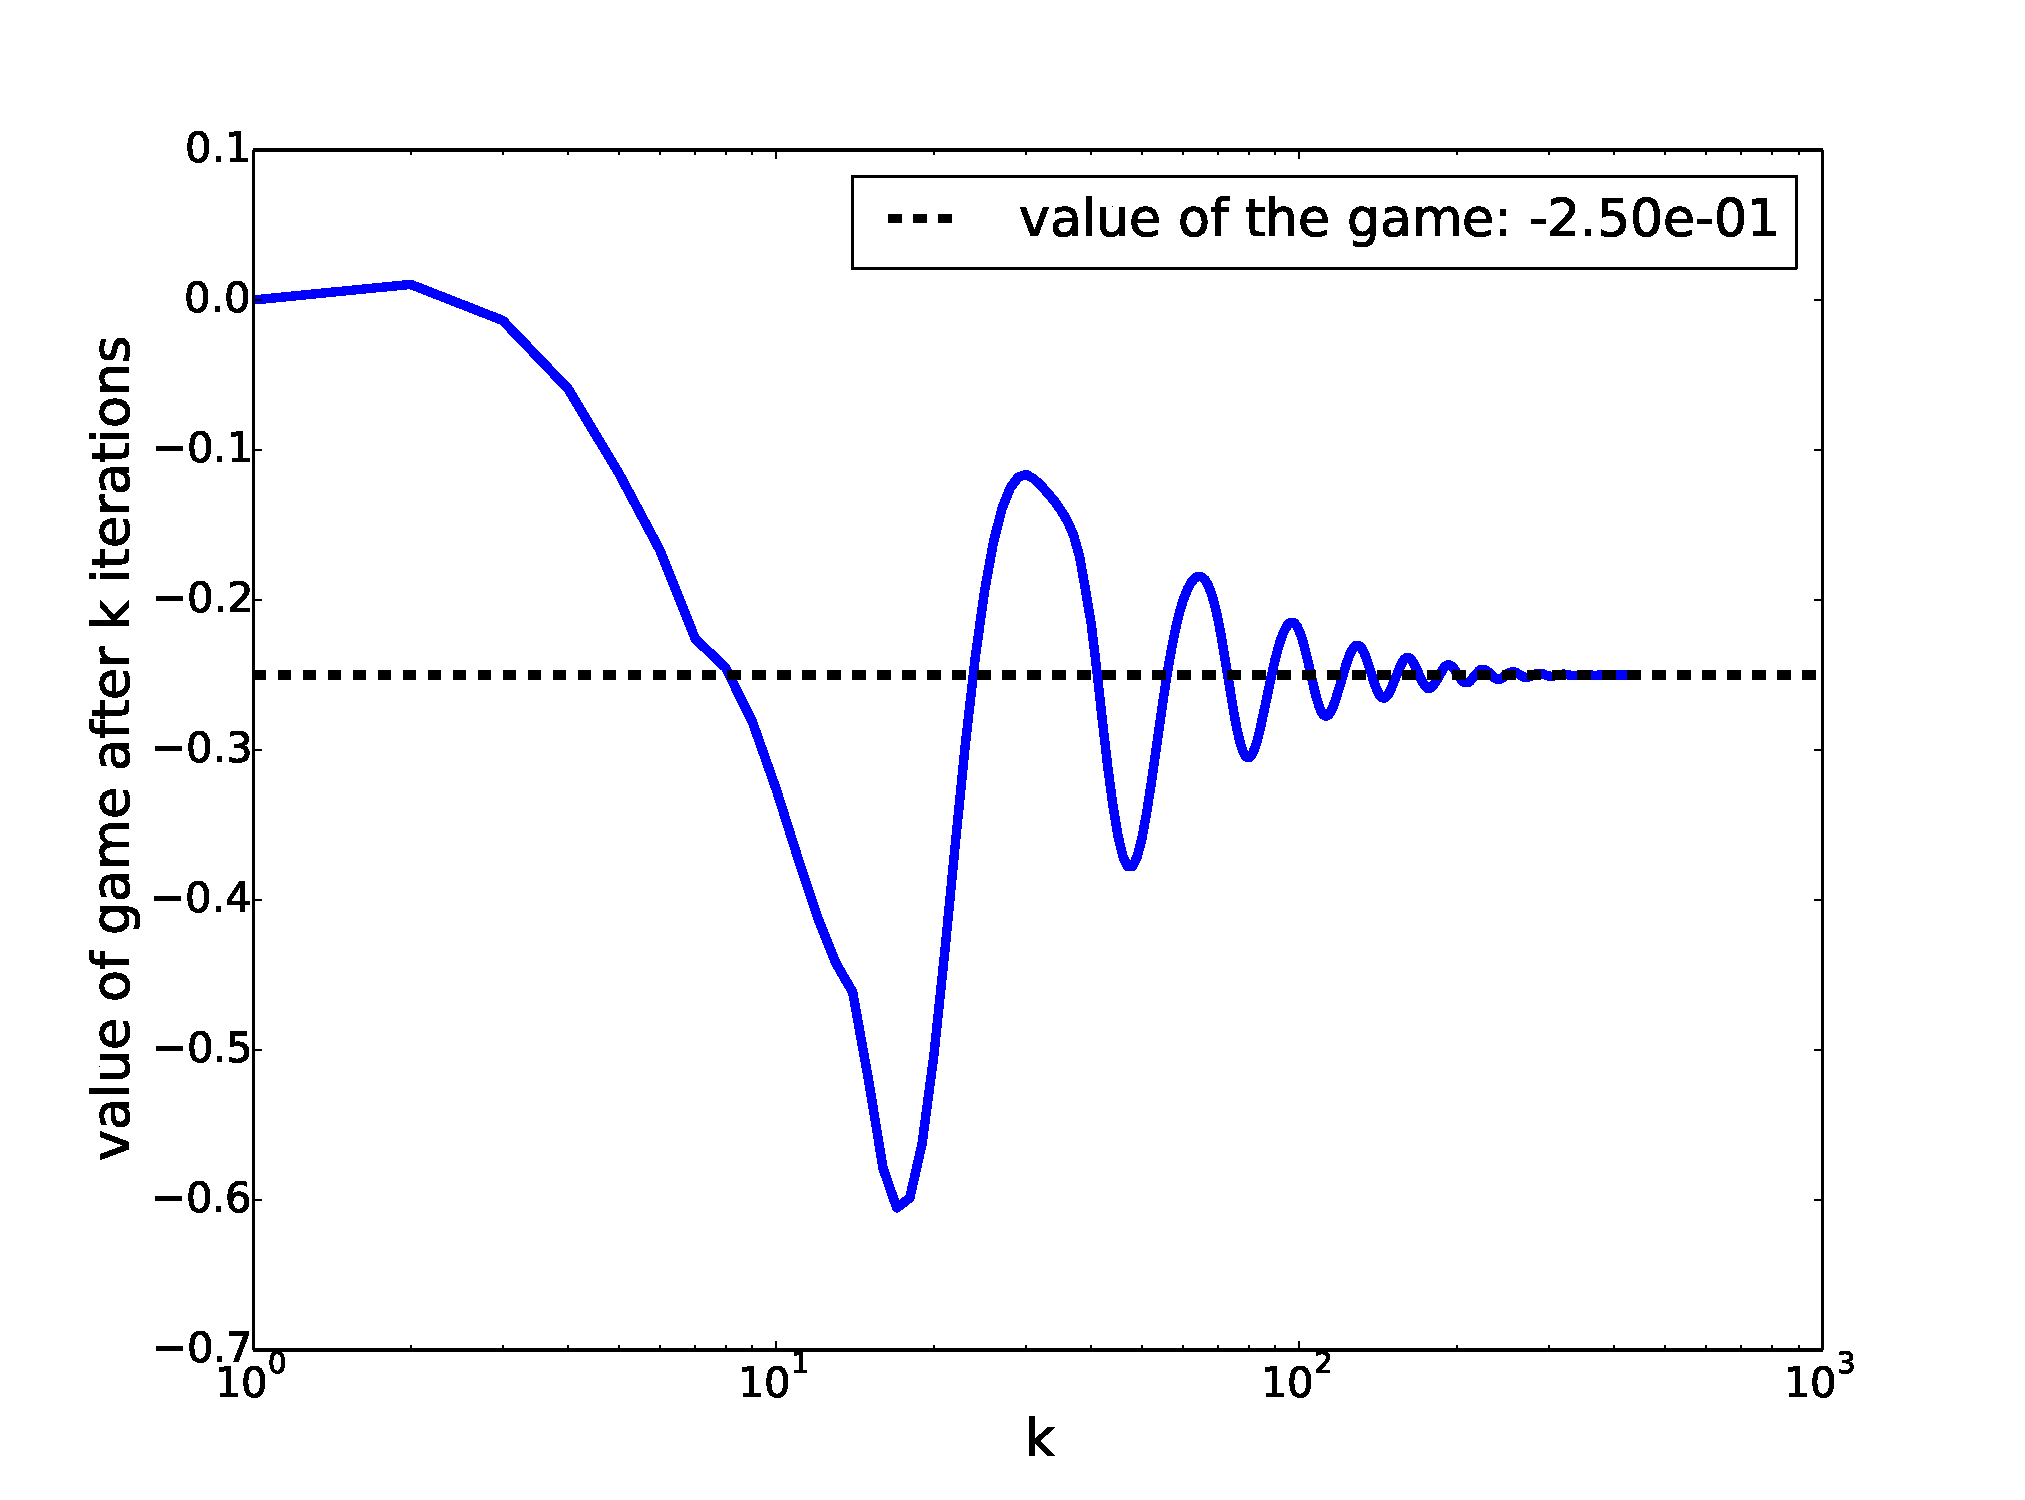
\includegraphics[width=.5\linewidth]{SimplifiedPoker_NE.pdf}
  \caption{Convergence curves of Algorithm \ref{Tab:algo_simplified} on simplified variants of Poker. \textbf{Left}: Kuhn Poker. \textbf{Right}: Another simplified Poker variant}.
  \label{Tab:conv_curves}
\end{figure}

\small
\bibliographystyle{ieeetr}
\bibliography{bib}


\end{document}
